\documentclass[tikz,border=5pt]{standalone}
\usepackage{tikz}
\usepackage{amsmath}
\usetikzlibrary{arrows.meta,positioning}
\definecolor{nebula}{HTML}{6366F1}
\definecolor{spark}{HTML}{14B8A6}
\definecolor{ink}{HTML}{334155}
\begin{document}
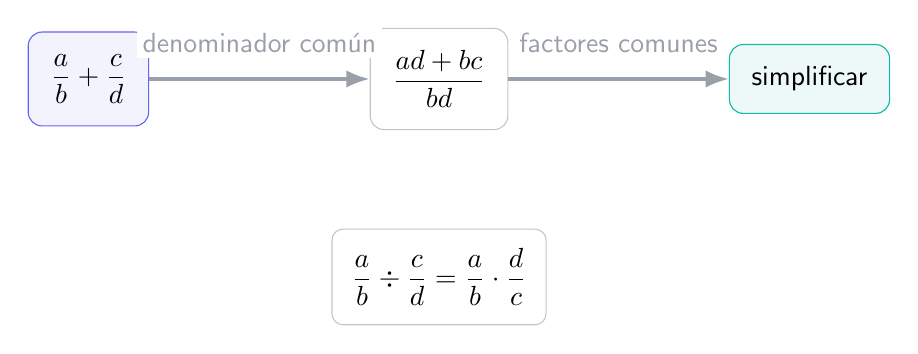
\begin{tikzpicture}[font=\sffamily,>=Latex,node distance=1.6cm]
  \node[draw=nebula,rounded corners=5pt,fill=nebula!8,inner sep=8pt] (a)
    {$\dfrac{a}{b}+\dfrac{c}{d}$};
  \node[draw=ink!30,rounded corners=5pt,fill=white,inner sep=8pt,right=2.8cm of a] (b)
    {$\dfrac{ad+bc}{bd}$};
  \node[draw=spark,rounded corners=5pt,fill=spark!8,inner sep=8pt,right=2.8cm of b] (c)
    {simplificar};
  \draw[->,very thick,ink!50] (a)--(b) node[midway,above=7pt,fill=white,inner sep=2pt] {denominador común};
  \draw[->,very thick,ink!50] (b)--(c) node[midway,above=7pt,fill=white,inner sep=2pt] {factores comunes};
  \node[draw=ink!30,rounded corners=4pt,fill=white,inner sep=7pt,below=1.25cm of b]
    {$\dfrac{a}{b}\div\dfrac{c}{d}=\dfrac{a}{b}\cdot\dfrac{d}{c}$};
\end{tikzpicture}
\end{document}
